\chapter{Binary Decision Diagrams}\label{ch-binarydd}

\begin{figure}[h!]
\centering
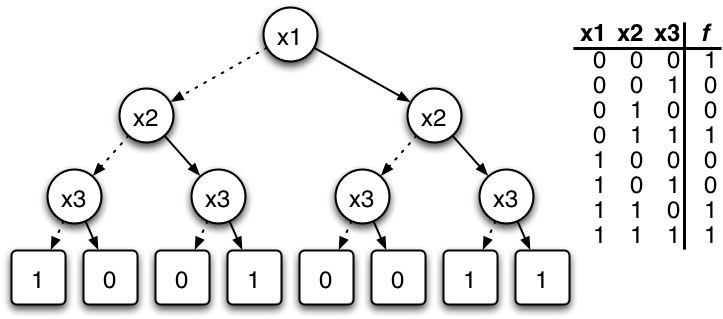
\includegraphics[width=4in]{binarydd/bdd-tree.png}
\caption{Binary decision tree and truth table 
for the function $
f(x_1, x_2,x_3)=
\bar{x}_1(x_2+\bar{x}_3)  + x_1 x_2 $ }
\label{fig-bdd-tree}
\end{figure}

\begin{figure}[h!]
\centering

\includegraphics[width=2.2in]{binarydd/bdd.png}
\caption{BDD for the function $f$
of Fig.\ref{fig-bdd-tree}.} 
\label{fig-bdd-bdd}
\end{figure}

This chapter is based
on Wikipedia article Ref.\cite{wiki-bdd}.

Binary Decision Diagrams (BDDs)
can be understood as a special
case of Decision Trees (dtrees).
We will
assume
that the reader has read
Chapter \ref{ch-dtree} 
on dtrees before
reading this chapter.



Both Figs.\ref{fig-bdd-tree}
and \ref{fig-bdd-bdd} were taken
from the aforementioned Wikipedia article. They
give a simple example of a function
$f:\bool^3\rarrow\bool$
represented in
Fig.\ref{fig-bdd-tree} as a
{\bf binary decision tree}
 and in Fig.\ref{fig-bdd-bdd} as a {\bf binary
decision diagram (BDD)}.
The goal 
of this chapter is
to find for each  of those 
figures a bnet with
the same graph structure.

We begin by noting
that the function
$f:\bool^3\rarrow\bool$
is a special case
of a probability
distribution
$P:\bool^3\rarrow[0,1]$.
In fact,
if we restrict $P$ to 
be deterministic, then
$P_{det}:\bool^3\rarrow\bool$
has the same domain
and range as $f$.
Henceforth,
we will refer to
$f(x_1,x_2,x_3)$
as $P(x_1,x_2,x_3)$,
keeping in mind that
we are restricting our
attention to deterministic
probability distributions. 

If we apply the chain
rule for conditional
probabilities to $P(x_1,x_2,x_3)$,
we get
\beq
P(x_1, x_2, x_3)=
P(x_3|x_1, x_2)P(x_2|x_1)P(x_1)
\;,
\eeq
which can be represented by the bnet:

\begin{figure}[h!]
$$
\xymatrix{
\rvx_1\ar[d]\ar@/^1pc/[dd]\\
\rvx_2\ar[d]\\
\rvx_3
}
$$
\caption{Most general 3 node bnet.}
\label{fig-bdd-3node-bnet}
\end{figure}




\begin{figure}[h!]
$$
\xymatrix{
\ul{x_1}\ar[d]\ar[drr]
\\
\ul{x_2|0}\ar[d]\ar[dr]
&&\ul{x_2|1}\ar[d]\ar[dr]
\\
\ul{x_3|00}\ar[d]\ar@/_2.5pc/[dd]
&\ul{x_3|01}\ar[d]\ar@/_2.5pc/[dd]
&\ul{x_3|10}\ar[d]\ar@/_2.5pc/[dd]
&\ul{x_3|11}\ar[d]\ar@/_2.5pc/[dd]
\\
\ul{x_4|000}
&\ul{x_4|010}
&\ul{x_4|100}
&\ul{x_4|110}
\\
\ul{x_4|001}
&\ul{x_4|011}
&\ul{x_4|101}
&\ul{x_4|111}
}
$$\caption{Image bnet for binary dtree
of Fig.\ref{fig-bdd-tree}.}
\label{fig-bdd-full-bnet}
\end{figure}

But
in Chapter \ref{ch-dtree},
we learned how
to represent
the dtree
of Fig.\ref{fig-bdd-tree}
as the image bnet
Fig.\ref{fig-bdd-full-bnet}.
The node TPMs, printed in blue,
for the image bnet Fig.\ref{fig-bdd-full-bnet}
are as follows.
Note that the TPMs for 
Fig.\ref{fig-bdd-full-bnet}
can be constructed from the
TPMs for the bnet Fig.\ref{fig-bdd-3node-bnet}.
If $x_1,x_2, x_3, x_4\in \{0,1,null\}$
and $a,b,c\in \bool$, then

\beq\color{blue}
P(\ul{x_1}=x_1)=
\left\{
\begin{array}{ll}
P_{\rvx_1}(x_1)&\text{if $x_1\in \bool$}
\\
0&\text{if $x_1=null$}
\end{array}
\right.
\eeq


\beq\color{blue}
P(\ul{x_2|a}=x_2\cond \ul{x_1}=x_1)=
\left\{
\begin{array}{ll}
P_{\rvx_2|\rvx_1}(x_2|a)&\text{if $x_1=a$}
\\
\indi(x_2=null)&\text{otherwise}
\end{array}
\right.
\eeq

\beq\color{blue}
P(\ul{x_3|a,b}=x_3\cond \ul{x_2|a}=x_2)=
\left\{
\begin{array}{ll}
P_{\rvx_3|\rvx_1,\rvx_2}
(x_3|a,b)&\text{if $x_2=b$}
\\
\indi(x_3=null)&\text{otherwise}
\end{array}
\right.
\label{eq-p-x3-x1x2}
\eeq

\beq\color{blue}
P(\ul{x_4|a,b,c}=x_4\cond \ul{x_3|a,b}=x_3)=
\left\{
\begin{array}{ll}
\delta(x_4,c)&\text{if $x_3=c$}
\\
\indi(x_4=null)&\text{otherwise}
\end{array}
\right.
\eeq

Note that if
$P_{\rvx_3|\rvx_1,\rvx_2}=
P_{\rvx_3|\rvx_2}$
in Eq.(\ref{eq-p-x3-x1x2}),
then the bnet Fig.\ref{fig-bdd-3node-bnet}
reduces to a Markov
 chain $\rvx_1\rarrow\rvx_2\rarrow\rvx_3$.



The BDD shown in
Fig.\ref{fig-bdd-bdd}
emphasizes the
fact that

\beq
P(x_1,x_2,x_3|x_1=1)=P(x_2|x_1=1)=x_2
\;.
\eeq
The BDD of Fig.\ref{fig-bdd-bdd}
has as image bnet
Fig.\ref{fig-bdd-simp-bnet}.
Define

\beq
pa(\ul{0})=pa(\ul{1})=(x_2|1, x_3|00, x_3|01)
\;.
\eeq 
Let $pa(\ul{0})=abc$ mean the same as
$pa(\ul{0})=(a,b,c)$.
The TPMs of the 
image bnet
Fig.\ref{fig-bdd-simp-bnet}
are the same as those for the
image bnet 
Fig.\ref{fig-bdd-full-bnet}
except for the TPMs of the
nodes $\ul{0}$
and $\ul{1}$.
For those two nodes, 
the TPMs, printed in blue,
are as follows.



\begin{figure}[h!]
$$
\xymatrix{
\ul{x_1}\ar[d]\ar[drr]
\\
\ul{x_2|0}\ar[d]\ar[dr]
&&\ul{x_2|1}\ar@/^2pc/[ddll]\ar@/^2pc/[dddll]
\\
\ul{x_3|00}\ar[d]\ar@/_1pc/[dd]
&\ul{x_3|01}\ar[dl]\ar[ddl]
&\bullet
&\bullet
\\
\ul{0}
\\
\ul{1}
}
$$
\caption{Image bnet for BDD of Fig.\ref{fig-bdd-bdd}.}
\label{fig-bdd-simp-bnet}
\end{figure}

\beq\color{blue}
P(\ul{0}=x|pa(\ul{0}))=
\left\{
\begin{array}{ll}
\delta(x,0) &\text{if $pa(\ul{0})=011$}
\\
\delta(x, null) &\text{otherwise}
\end{array}
\right.
\eeq

\beq\color{blue}
P(\ul{1}=x|pa(\ul{1}))=
\left\{
\begin{array}{ll}
\delta(x,1) &\text{if $pa(\ul{1})=101$}
\\
\delta(x, null) &\text{otherwise}
\end{array}
\right.
\eeq
